% For some reason pdflatex says it can't find this file, then i type "X" and it works
% also you have to compile it twice to get the png
\documentclass[preview, convert={density=300,size=1080x800,outext=.png}]{standalone}
\usepackage{caption}
\usepackage{tikz}
\usepackage{tkz-graph}

\SetVertexNormal[Shape      = circle,
                 FillColor  = orange,
                 LineWidth  = 2pt]
\SetUpEdge[lw         = 0.5pt,
           color      = black,
           labelcolor = white,
           labeltext  = red]


\begin{document}
\begin{figure}
    \centering
    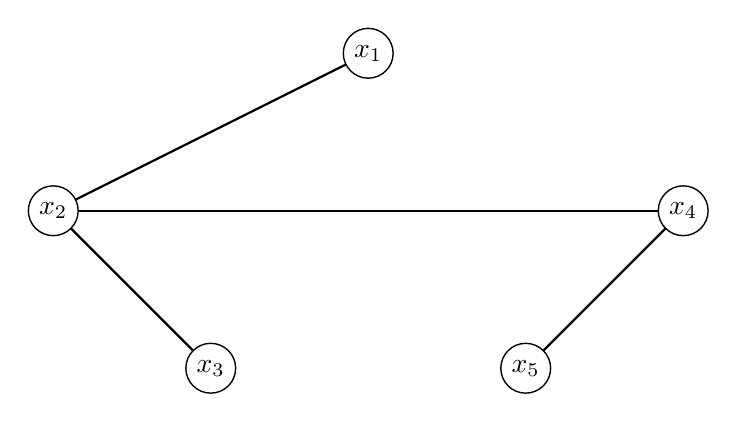
\begin{tikzpicture}
        \Vertex[ x=0, y=0, L=$x_1$]{x1}
        \Vertex[ x=-4, y=-2, L=$x_2$]{x2}
        \Vertex[ x=-2, y=-4, L=$x_3$]{x3}
        \Vertex[ x=4, y=-2, L=$x_4$]{x4}
        \Vertex[ x=2, y=-4, L=$x_5$]{x5}

        \Edge(x1)(x2)
        \Edge(x2)(x3)
        \Edge(x2)(x4)
        \Edge(x4)(x5)
    \end{tikzpicture}
    \caption*{An example of a dependency tree}

\end{figure}
\end{document}
